\section{Theorie}
\label{sec:Theorie}

\subsection{Theoretische Grundlagen zum Photoeffekt}
\label{subsec:Theorie_Photoeffekt}

Der Photoeffekt beschreibt die Auslösung von Elektronen aus Oberflächen von Metallen
durch Bestrahlung mit Licht. Die Erklärung der im Folgenden noch zu erläuternden
Beobachtungen ist nur durch ein Korpuskelmodell möglich. Dieses besagt, dass sich
Licht in einzelnen sogenannten Photonen oder auch Lichtquanten fortbewegt, die nach
Einstein identisch mit Planck'schen Energiequanten sind.

Um eindeutige Beobachtungen machen zu können, wird beim Photoeffekt eine Festkörperfläche
im Vakuum mit monochromatischem Licht bestrahlt. Diese wird auch Photokathode genannt.
Der Photokathode gegenüber steht eine Auffängerelektrode mit positivem Potential.
Die Photokathode und die Auffängerelektrode sind über ein Strommessgerät miteinander verbunden.
Eine Skizze zu diesem Aufbau befindet sich in Abbildung \ref{fig:photoeffekt_skizze}.

\begin{figure}
  \centering
  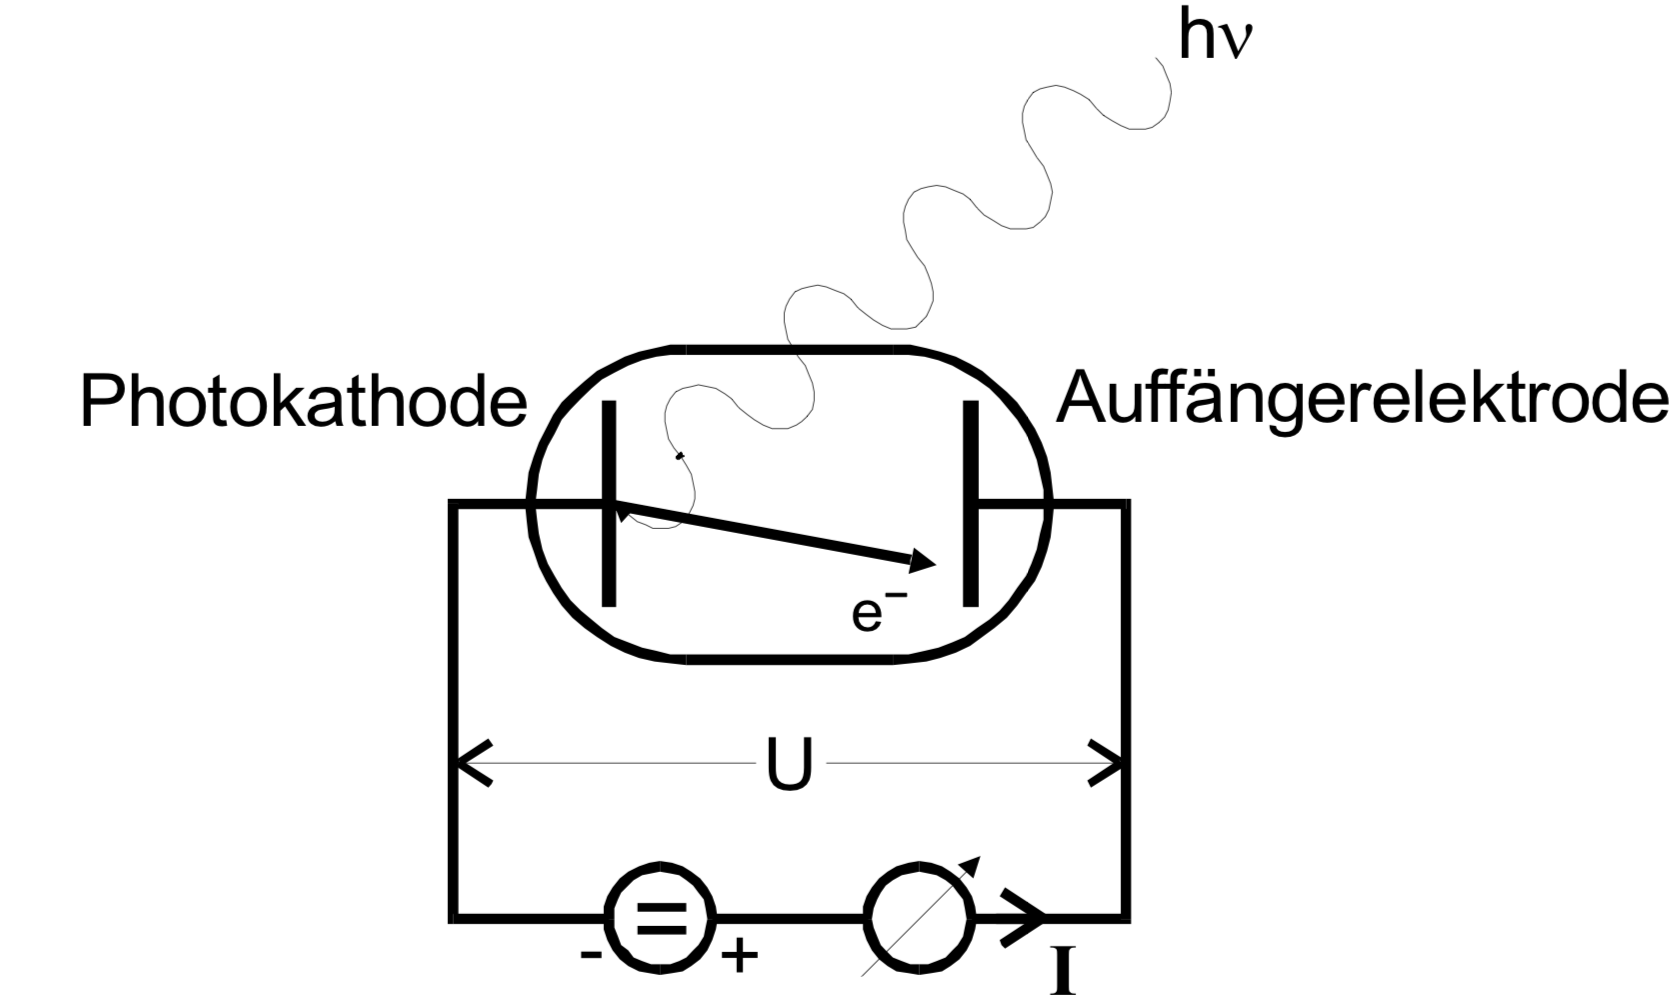
\includegraphics[height=4cm]{data/photoeffekt_skizze.png}
  \caption{Skizze für den grundelgenden Aufbau des Versuchs zum Photoeffekt \cite{Versuchsanleitung}.}
  \label{fig:photoeffekt_skizze}
\end{figure}

Wird die Festkörperfläche nun mit monochromatischem Licht bestrahlt, so treten aus dieser
Elektronen aus, die durch das elektrische Feld zur Auffängerelektrode gelangen, sodass
ein Strom, der sogenannte Photostrom gemessen werden kann. Im Wesentlichen lassen
sich drei Beobachtungen machen.

Die Anzahl der pro Zeitintervall ausgelösten Elektronen ist proportional zu der
Lichtintensität. Eine Erklärung hierfür besteht darin, dass die Intensität im Korpuseklmodell
durch die Anzahl der Photonen in einem bestimmten Raumwinkelanteil definiert ist.
Eine höhere Lichtintensität bedeutet also mehr Photonen, die entsprechend auch mehr
Elektronen auslösen können.

Eine weitere Beobachtung ist, dass die Energie der Photoelektronen, auf deren Messung später noch
eingegangen wird, proportional zu der Frequenz des Lichtes und nicht Abhängig von der
Intensität ist. Dies ist dadurch zu erklären, dass ein Elektron im Festkörper ein Photon
immer nur als Ganzes absorbieren kann, also nur die gesamte Energie des Photons auf ein mal
Aufnehmen kann. Die Energie eines Photons ist definiert als
\begin{equation}
  E=h f \,.
\end{equation}
Somit ist auch der Zusammenhang der Energie der Photoelektronen zur Frequenz des Lichtes gegeben.

Die Beobachtung, dass der Photoeffekt nur oberhalb einer Grenzfrequenz auftritt, lässt sich
durch die Existenz einer Austrittsarbeit $A_{\symup{k}}$ erklären. Die Energie der
Photoelektronen ergibt sich zu
\begin{equation}
  h f= E_{\symup{kin}}+A_{\symup{k}} \,.
\end{equation}
Somit können Elektronen, auf die nur eine Energie $E=hf<A_{\symup{k}}$ übertragen wird
nicht mehr austreten, sodass auch kein Photoeffekt zustande kommt.

\subsection{Theoretische Grundlagen zur Messmethode}
\label{subsec:Theorie_Messung}

Um die Energie der Photoelektronen zu messen, wird die Gegenfeldmethode verwendet. Ein
Schaltbild für diese befindet sich in Abbildung \ref{fig:schaltbild}. Zwischen
Kathode und Anode wird ein elektrisches Feld angelegt, das die Elektronen abbremst.
Gleichzeitig wird der Photostrom gemessen. Dieser verschwindet genau dann, wenn
\begin{equation}
  e_0 U_{\symup{g}}=\frac{m_0 v_{\symup{max}}^2}{2}
\end{equation}
gilt. Dabei ist $U_{\symup{g}}$ die Gegenspannung und $v_{\symup{max}}$ die
Geschwindigkeit der schnellsten Elektronen. $e_0$ und $m_0$ sind die Ladung und die
Masse eines Elektrons. Die Energie der schnellsten Elektronen folgt dem Zusammenhang
\begin{equation}
  h f=e_0 U_{\symup{g}} + A_{\symup{k}} \,.
\end{equation}

\begin{figure}
  \centering
  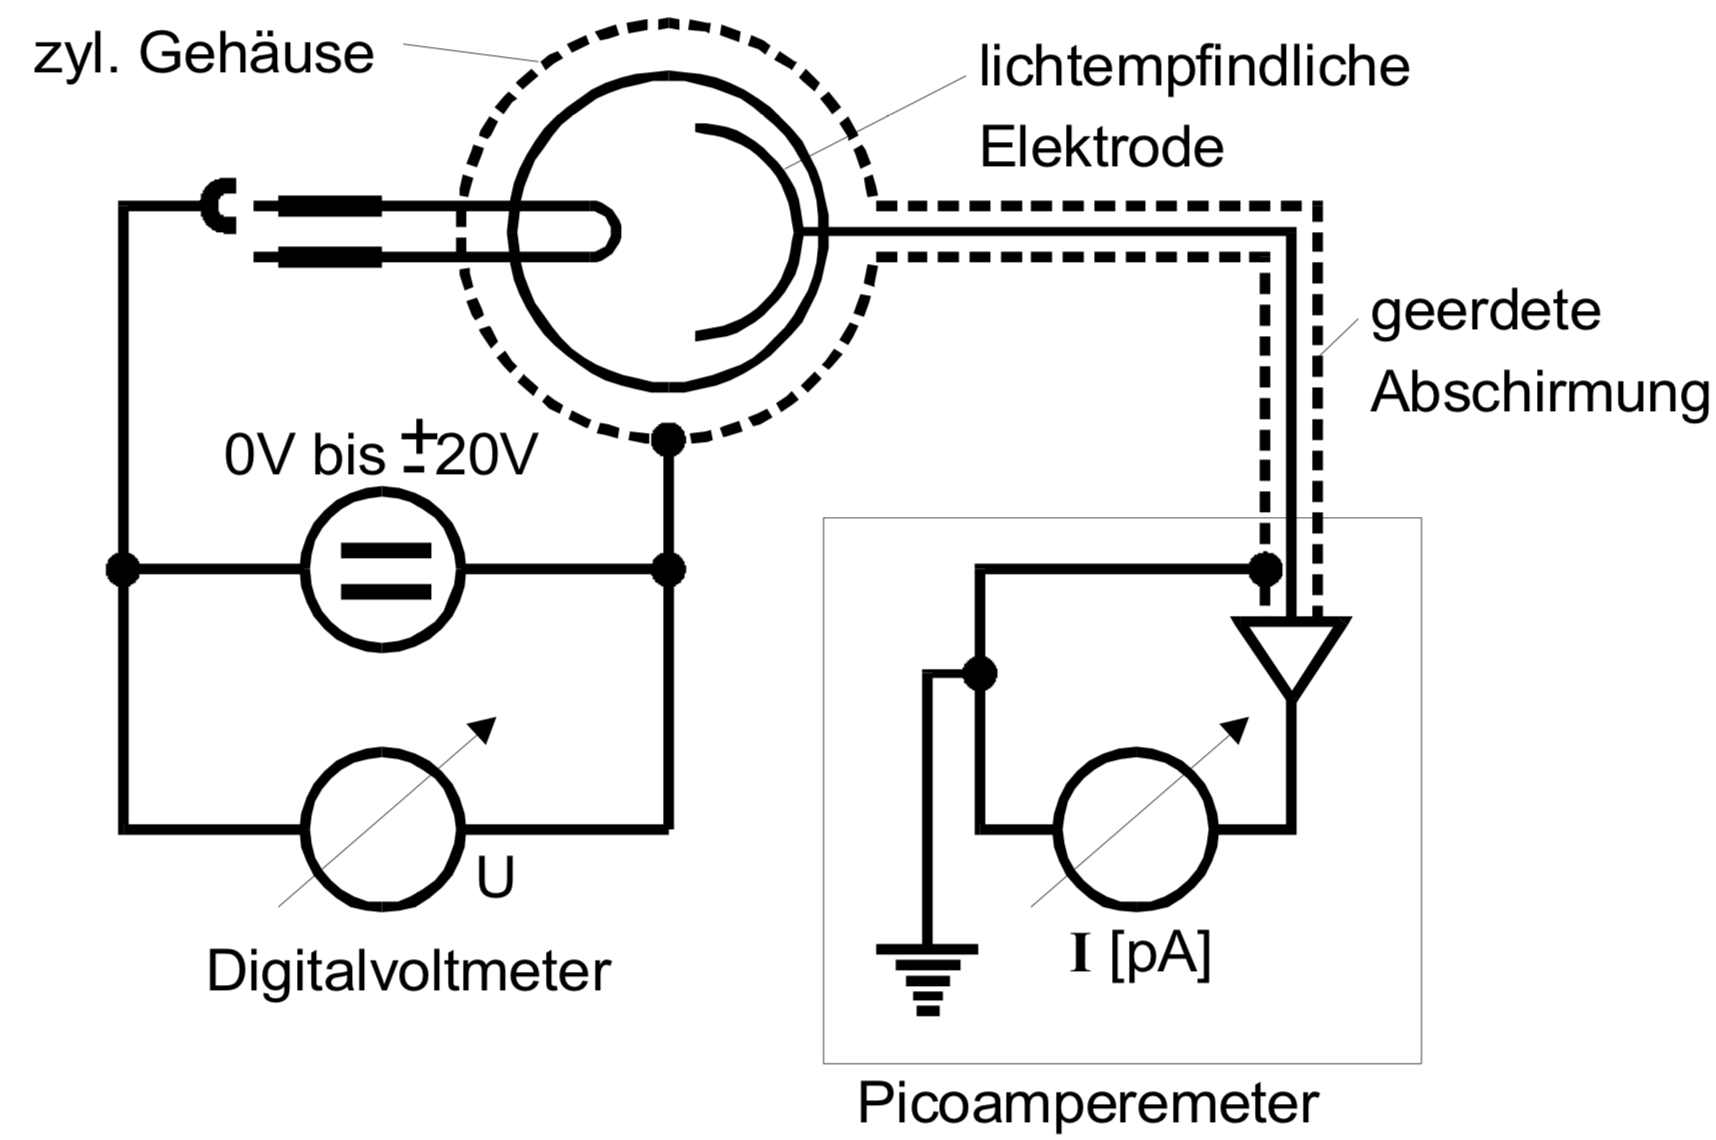
\includegraphics[height=4cm]{data/schaltbild.png}
  \caption{Schaltbild für die Messung der Elektronenenergien mithilfe der Gegenfeldmethode \cite{Versuchsanleitung}.}
  \label{fig:schaltbild}
\end{figure}

Der Photostrom in Abhängigkeit von der Gegenspannung, der im Experiment beobachtet werden kann,
folgt jedoch dem in Abbildung \ref{fig:photostrom} dargestellten Verlauf. Es ist
auffällig, dass der Photostrom nicht erst bei der einer bestimmten Gegenspannung $U_{\symup{g}}$
plötzlich auf null abfällt, sondern kontinuierlich sinkt. Dies ist so, da die Energie der
Elektronen von ihrem Zustand im Festkörper abhängt. Durch diesen Zusammenhang wird die
Bestimmung der Gegenspannung, bei der kein Strom mehr fließt, deutlich erschwert.
Unter bestimmten in diesem Versuch gegebenen Voraussetzungen zeigt sich jedoch der
Zusammenhang
\begin{equation}
  I_{\symup{ph}} \propto U^2 \,.
  \label{eqn:iu2}
\end{equation}

\begin{figure}
  \centering
  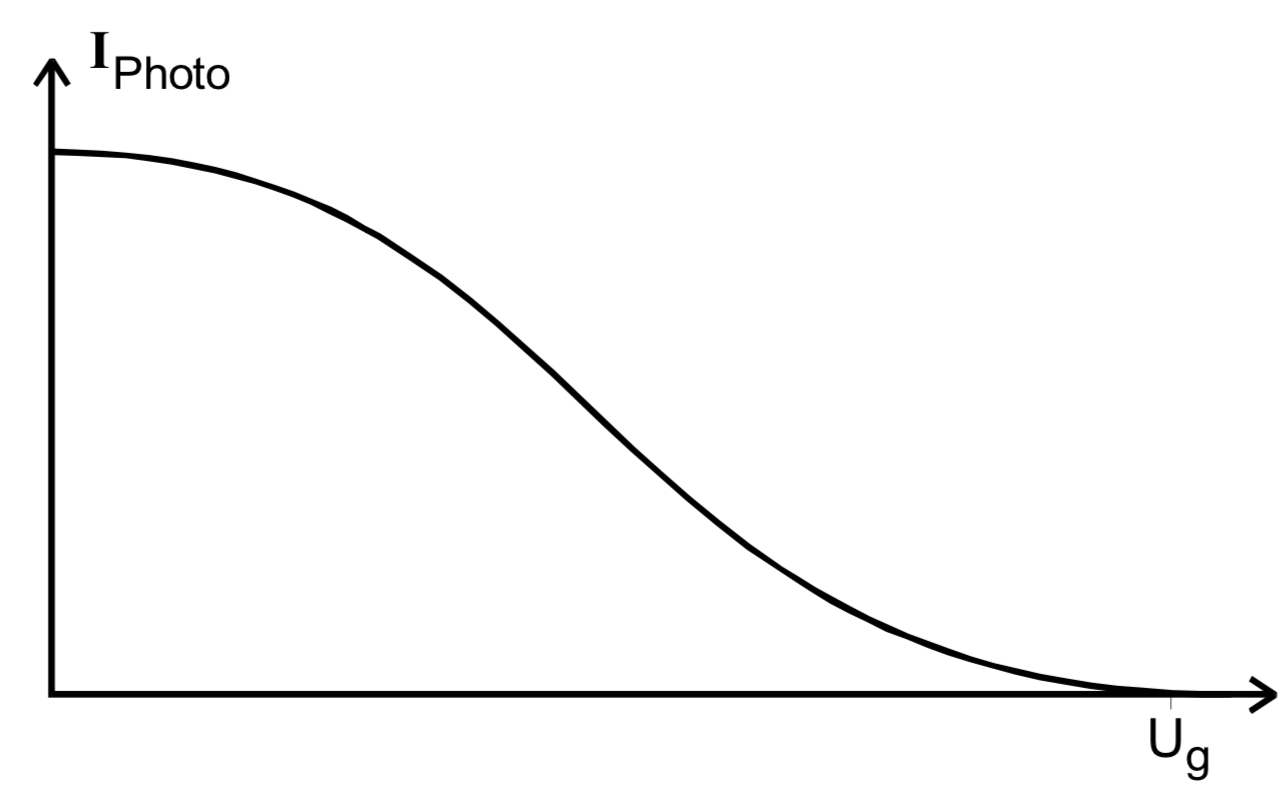
\includegraphics[height=4cm]{data/photostrom.png}
  \caption{Verlauf des Photostroms in Abhängigkeit von der Gegenspannung \cite{Versuchsanleitung}.}
  \label{fig:photostrom}
\end{figure}

Ein weiterer Faktor, der die Messung erschweren kann, tritt auf, wenn das Anodenmaterial
eine Austrittsarbeit $A_{\symup{A}}$ besitzt, die größer ist, als die Energie $E=hf$ der
Photonen. Dann müssen die Elektronen vor dem Erreichen der
Anode ein Gegenfeld durchlaufen. Das kann dazu führen, dass kein Photostrom auftritt.
In diesem Fall muss eine Beschleunigungsspannung $U_{\symup{b}}$ angelegt werden.
Ein Photostrom ist erst dann messbar, wenn
\begin{equation}
  hf + e_{\symup{0}}U_{\symup{b}}≥A_{\symup{A}}
\end{equation}
erfüllt ist.
